\label{chapter:tool}
This section presents \toolname, a \textit{java-based} tool aimed at helping  developers during the testing process of their Android mobile applications. The tool is composed by a set of sub-components that operate sequentially. The first one is the component that is charge to exercise the SUT, revealing and collecting crashes. The second component processes the gathered data, as explained in Section \ref{approach:clustering}. At the end, the tool is able to recommend traceability links between the stack traces and a set of mined user reviews for the same app under test. The chapter follows with a technical description of the implemented components, as well with the instructions to run the tool.


\section{Testing Component}
\label{tool: testing}
%----------------- FDROID CRAWLER --------------
First of all, if no set of \textit{APKs} is available yet, \toolname\ can be exploited for downloading the needed mobile applications from the \textit{F-Droid API\footnote{https://f-droid.org/repo/}}. In this direction, as shown in the picture \ref{testing}, the component \FDroidCrawler, is first in charge of  parsing a static structured file (\textit{e.g.} a \textit{csv} file) that contains a set of Android packages names that univocally represent a given app of the Google Play Store. 
The path of this file is given in the \textsc{ConfigurationManager}, which contains a set of static properties that get elaborated by \toolname. Second, \textsc{FdroidCrawler} searches and then extracts a set of \textit{HTTP links} for those android packages that have been found on the API. Afterwards, it builds the correct \textit{HTTP requests} and finally starts the downloading process, saving the returned \textit{APKs} in a given directory.

%-------------- CONFIGURATION ENVIRONMENT--------------
The first step of the testing part was to build a set of \textit{APKs}, with which to perform the testing process. As said, this can be achieved using either \textsc{FdroidCrawler} or can also be manually created. Now, the second step is to prepare and configure the testing environment. 
All the parameters needed for starting a testing session have to be specified in the \textsc{ConfigurationManager}. Figure \ref{lst: config}, shows an example of a simplified set of parameters which must be given a priori in order to launch a testing session. \newpage
\label{lst: config}
\begin{lstlisting}[caption=Properties which get elaborated during the testing sessions,label={lst: config}]
/**
* Dataset directories
*/
CSV_FILE_DIR = Dataset/dataset.csv
APK_DIR = Downloads/apks 

/**
* Test logs directories
*/
MONKEY_DIR = Reports/MonkeyReports
SAPIENZ_DIR = Reports/SapienzReports

/**
 * Testing session specifications
 */
MINUTES_PER_APP = 30
NR_OF_ITERATIONS = 5

/**
 * Monkey parameters
 */
LOG_VERBOSITY = -v 
PACKAGE_ALLOWED = -p
NR_INJECTED_EVENTS = 5000
DELAY_BETWEEN_EVENTS = 10
PERCENTAGE_TOUCH_EVENTS = 15
PERCENTAGE_SYSTEM_EVENTS = 15
PERCENTAGE_MOTION_EVENTS = 15
IGNORE_CRASH = True

/**
* Sapienz parameters
*/
SEQUENCE_LENGTH_MIN = 20
SEQUENCE_LENGTH_MAX = 500
SUITE_SIZE = 5
POPULATION_SIZE = 50
OFFSPRING_SIZE = 50
GENERATION = 100
CXPB = 0.7
MUTPB = 0.3
\end{lstlisting}
The figure above represents a part of the \textsc{ConfigurationManager}, where all the testing parameters for \monkey and \sapienz are specified (\textit{line 22-41}). An in-depth explanation about these parameters concering \monkey and \sapienz can be found in the section \ref{usage: settings}.
Furthermore, the directories containing the dataset must be specified. These include the location of the static structured file and the directory where the \textit{APKS} are going to be stored (\textit{line 4-5}).
In addition to them, the directories on which the generated test logs are going to be saved (\textit{line 10-11}) as well as the specifications about the testing session (\textit{line 16-17}) must be given. 
The tool accepts two parameters that tune the duration and the execution of the tests:
\begin{itemize}
\item \textsc{minutes\_per\_app}, specifies how many minutes an app will be tested. After that time frame, a time-out occurs and the testing process gets restarted with the next app. 
Referring to the approach explained in the section \ref{approach:testing}, this value represents the  \textit{single app} testing cycle.
\item \textsc{nr\_of\_iterations}, specifies how many times the whole dataset will be tested.
This value, in turn, describes the \textit{session cycle}.
\end{itemize}

According to the example \ref{lst: config} above and assuming that the dataset consists in 10 apps, the total estimated testing time for an entire testing session would be: 
\begin{align*}
30 \:min \: \frac{per}{app} * 10\: app * 5\: iterations = 1500 \:min. \:(25\: hours). 
\end{align*}
Once the testing environment has been configured, the automated tool with whom the testing is going to be performed must be made explicit. 
Indeed, it has to be specified as parameter in \textsc{main} \textit{args} (as mentioned before in the section \ref{sec:choicetool}, the tool which can be selected is either \monkey or \textsc{Sapienz}).

The last configuration step is to define on which kind of device (\textit{i.e}, a real device, such as a \textit{tablet} or a virtual device, such as an \textit{emulator}) the testing is going to be performed. In addition to them, an additional argument that starts a timer for a better overview during the testing process can also be passed as main argument. \toolname\ supports different types of emulators or real devices running on different android API levels. However, in order to correctly execute \sapienz, the API level shall be \textit{Android 4.4, KitKat}. \\
The listing below shows an example of a possible combination of parameters that could be given as main arguments. 
\begin{lstlisting}[caption=Possible \toolname\ command line, language=bash]
$ java -jar BECLOMA.jar -device -monkey -timer
\end{lstlisting}
Section \ref{usage: settings} describes the full usage of \toolname. 

%-----------LAUNCH A TESTING SESSION -----------
\paragraph{Session cycle.} Once the configuration phase is terminated, \toolname\ is able to start concrete the testing process. 
As shown in the picture \ref{testing}, it manages the component \SessionLauncher, which is in charge of translating the previously specified testing properties into "java readable code" and initializing the \textit{session cycle} mentioned in the approach. 
Concretely, after \toolname\ invokes \SessionLauncher\ all attached devices respectively the chosen emulators get initialized, \ie they get rebooted and restarted as root, so that some important write-read-permissions are enabled during the testing session. 
Whether the timer has been given as main argument, it gets also started. \\
Once the initialization step has been completed, \SessionLauncher\  invokes the \AppTester\ component which is in charge of starting the \textit{dataset cycle}. The Listing~\ref{lst:startsession} gives a simplified code snippet about the beginning of this testing cycle. 
\clearpage
\begin{lstlisting}[caption=\SessionLauncher\ Code snippet for starting a testing session ,label={lst:startsession}]
private appTester; 
public void startTestingSession() throws Exception {
        final int NUMBER_ITERATIONS = ConfigurationManager.getNumberOfIterations();
        if (IS_EMULATOR) {
        	   SessionLauncher.initialiseEmulator();
        }
        else {
       	   SessionLauncher.initialiseDevices();
        }
       
        if (isTimer) {
            SessionLauncher.initializeTimer();
        }
        for (int i = 0; i < NUMBER_ITERATIONS; i++) {
            System.out.println("Iteration number " + (i+1));
            this.appTester = new AppTester();
            this.appTester.testAllApp();
        }
}
\end{lstlisting}
First of all, the total number of iterations specified in the \Config\ is read and stored into a constant of type int. After that, the specified device gets initialized, statically invoking the correspondent method (\textit{line 4-9}).  
According to the boolean variable \textit{isTimer}, a timer may also be started (\textit{line 11-13}).
Afterwards, a for-loop starts, where at each iteration the method \textit{testAllApp()} gets invoked. 
Referring to the approach explained in the section \ref{approach:testing}, at each iteration a new object of type \AppTester\ is created, which represents exactly one \textit{dataset cycle}. 
As shown in the figure~\ref{testing}, the \SessionLauncher\ would be able to instantiate infinite times the class \AppTester. However, it must create at least one object of that type in order to start a testing session. 

\paragraph{Dataset and single app cycles. } 
\AppTester\ and \Cmd\ represent the core components of the whole testing process. Indeed, \AppTester\ can be viewed as brain of the process, since it tells step-by-step to the body, \ie the \Cmd\ component, which commands it has to execute and at what stage of the process it has to perform it. \\
Listing~\ref{lst:apptester} shows a very simplified code snippet of the relation between the two above mentioned components. 


First of all, \AppTester\ creates a for-loop in which it iterates each \textit{APK} file contained in the \textit{APKs} directory. Once again, this directory is specified in the \Config. 
The first if statement checks whether the file in question has an adequate extension, \ie it is able to be installed on a android mobile device. 
After that, \AppTester\ uninstalls the concerned \textit{APK}, so that at each iteration of the testing it gets reinstalled. 
This beacause, it may be that an \textit{APK} gets affected by some previously generated sequences (\eg a sequence of random events that led the app to an external website). \\
Afterwards, \AppTester\ checks which automated tool has been chosen by the tester, so that it can tell to the \Cmd\ component, which command-line it has to execute. As stated before, \AppTester\ prepares the single testing components such as which \textit{APK}, which tool, which testing parameters, etc., while \Cmd\ executes them without any prior knowledge. \\

\clearpage
\begin{lstlisting}[caption=Testing mechanism between \AppTester\ and \Cmd\, ,label={lst:apptester}]
/**
* @class: AppTester
*/
public void testAllApp() {
        for (File apk : this.apksDirectory) {
            if (apk.getName().endsWith(".apk") && !apk.isDirectory()) {
                    uninstallApp(apk.getName());
                    installApp(apk.getName());
                    if (IS_MONKEY) {
                        testAppWithMonkey(config.getMonkeyRepDir(), apk.getName());
                    } else if (IS_SAPIENZ) {
                        testAppWithSapienz(config.getSapienzRepDir(), apk.getName());
                    }
            }
        } 
        // waiting to threads to finish 
        File testLog = CmdExecutor.getCurrentLog();
        if (hasCrash(testLog)) {
            generateCrashLog(testLog);
        }
} 
private void testAppWithSapienz(String dest, final String APK_NAME) {
	CmdExecutor.generateReport(dest, CommandLines.SAPIENZ_CMD_LINE(APK_NAME)); 
}

private void testAppWithMonkey(String dest, final String APK_NAME) {
	CmdExecutor.generateReport(dest, CommandLines.MONKEY_CMD_LINE(APK_NAME)); 
}

/**
* @class: CmdExectutor
*/
public static void generateReport(String dest, String cmd){
        Runtime runtime = Runtime.getRuntime();
        Process p = runtime.exec(cmd);
        StreamGobbler output = new StreamGobbler(p.getInputStream(), cmd, dest); 
        output.start();
        writeTestingEndTime(dest);
    }
    
public static File getCurrentLog() {
    return lastGeneratedLog();
}
    
\end{lstlisting}
\clearpage 
Once the automated tool has been detected, \Cmd\ is able to concretely start the \textit{single app cycle}, executing the passed command-line. This is represented in listing \ref{lst:apptester} by the method \textit{generateReport} (\textit{line 33}). Indeed, \Cmd\ uses a single instance of the java-class \textit{Runtime} that allows the application to interact with the environment in which the app is running \cite{runtime}. 
This is actually achieved by the \textit{Runtime.getRuntime()} (\textit{line 34}). The next line concretely executes the passed command-line. 
The returned code of the function call at \textit{line 35} consists of a new \textit{process} object. 
The process actually contains the execution of the command line. 
Assigning the execution of each single command-line to a new single separate process has advantages; In particular: 
\begin{itemize}
\item Processes are independent to each other. 
Whether the execution of a command-line fails, it can be interrupted without affecting the entire testing process; 
\item Multithreading can be easily supported; Indeed, the component \Stream\ extends the \textit{Thread} java-class which implements the \textit{Runnable} java-interface. Each time a new process comes in, it starts a new thread in this class.
\item Each process has it own timeout. It may be that some command-lines cannot properly terminate and need to be interrupted during their execution.  
\end{itemize}
\paragraph{Reporting phase.}
\Stream, in turn, is in charge of writing the test report. Each time its constructor get instantiated in the \textit{generateReport()} method in the \Cmd\ class, it starts a new thread and begins in parallel the writing phase of the log. 
As shown in listing~\ref{lst:gobbler}, the method \textit{run()} overrides the method located in the \textit{Runnable} interface. 
Indeed, it gets automatically invoked when in the \textit{generateReport()} method an object of type \textit{StreamGobbler} calls the function \textit{start()}  (\textit{line 37}). 
Once it gets called, the \textit{reporting} phase begins. This phase uses a \textit{PrintWriter} as well as classic \textit{Reader} for writing text on a file.
Before the test log is written, the metadata about the testing environments are appended to the writer. At the end of the process the writer is closed and the thread can terminate. Once the thread is finished, the method \textit{writeTestingEndTime()} (\textit{line 38}) can be executed.  
It complements the metadata, writing the testing end time, so that the total testing time can be computed. 





\begin{lstlisting}[caption=\Stream\ code snippet writing a test log, ,label={lst:gobbler}]
/**
* @class: StreamGobbler
*/
@Override
public void run() {
        try {
            Writer writer = new PrintWriter(outputPath, "UTF-8");
            InputStreamReader isr = new InputStreamReader(is);
            BufferedReader br = new BufferedReader(isr);
            String line;
            writer.append(TesterData.getMetaData()); // insert metadata
            while ((line = br.readLine()) != null) {
                System.out.println(" > " + line); // console overview
                writer.append(line).append("\n"); // test log 
            }
            closeWriter();
        } catch (IOException ioe) {
            ioe.printStackTrace();
        }
}
\end{lstlisting}

Listing~\ref{lst:testinglog} shows a short version of a test log of the app \textit{com.danvelazsco.fbwrapper} that has been generated after the execution of \monkey. 

\begin{lstlisting}[caption=Test log of com.danvelazco.fbwrapper, basicstyle=\fontsize{7}{8}\ttfamily,label={lst:testinglog}]
/**
 * Meta-data
 */
Tester Name: Lucas Pelloni
Testing Start Time: 05/04/2017 11:18:29
Testing End Time: 05/04/2017 11:48:30
Total Testing Time: 30 minutes (0.5 hours)
Type of testing: testing on a physical device
Device name: c0808bf731ab321
Percentage of motion events: 2.0% (number of motion events: 60 of 3000 events)
Percentage of system events: 6.0% (number of system events: 180 of 3000 events)
Percentage of touch events: 1.0% (number of touch events: 30 of 3000 events)

/**
 * Test log 
 **/
:Monkey: seed=1495075565065 count=3000
:AllowPackage: com.danvelazco.fbwrapper
:IncludeCategory: android.intent.category.LAUNCHER
:IncludeCategory: android.intent.category.MONKEY
// Event percentages:
//   0: 1.0%
//   1: 2.0%
//   2: 2.4931507%
//   3: 18.698631%
//   4: -0.0%
//   5: 31.164383%
//   6: 18.698631%
//   7: 6.0%
//   8: 2.4931507%
//   9: 1.2465754%
//   10: 16.205479%
:Switch: #Intent;action=android.intent.action.MAIN;category=android.intent.category.LAUNCHER;end
    // Allowing start of Intent { act=android.intent.action.MAIN cat=[android.intent.category.LAUNCHER]
:Sending Trackball (ACTION_MOVE): 0:(4.0,4.0)
:Sending Trackball (ACTION_MOVE): 0:(4.0,-3.0)
:Sending Trackball (ACTION_MOVE): 0:(2.0,-1.0)
:Sending Trackball (ACTION_MOVE): 0:(-5.0,2.0)
:Sending Trackball (ACTION_MOVE): 0:(-5.0,3.0)
    //[calendar_time:2017-05-05 09:48:23.894  system_uptime:717348]
    // Sending event #100
...
\end{lstlisting}

As shown in the figure above, the test logs do not only contain the test results of the tested app, but also the above mentioned meta-data for documenting and retracing the whole testing session.

\paragraph{Investigating phase. }
The \textit{single app cycle} in the "strict sense", \ie the stage where the \textit{APK} gets stressed with an automated tool is over. At this point, the logs must be investigated about the possibility that some apps have generated a crash during its testing time frame. In this sense, the last part of the method \textit{testAllApp()} illustrated in the listing ~\ref{lst:apptester}, is in charge of stating whether a test log contains a crash or not. The method for checking whether a test log has collected a crash inside it is quite intuitive. This because, the syntax used by \monkey and \sapienz in their report for indicating the presence of a crash is the same. As illustrated in the listing~\ref{lst:crashlog}, a crash can be delimited using the following two \textit{Strings}: 
\begin{itemize}
\item Crash beginning: \texttt{"// CRASH: "}
\item Crash end: \texttt{"// "}
\end{itemize}

\begin{lstlisting}[caption=Crash log of com.danvelazco.fbwrapper illustrated within its test log, basicstyle=\fontsize{6}{8}\ttfamily,label={lst:crashlog}]
...
:Sending Trackball (ACTION_MOVE): 0:(3.0,3.0)
:Sending Trackball (ACTION_MOVE): 0:(-4.0,-3.0)
:Sending Trackball (ACTION_MOVE): 0:(3.0,-1.0)
// CRASH: com.danvelazco.fbwrapper (pid 4302)
// Short Msg: java.lang.NullPointerException
// Long Msg: java.lang.NullPointerException
// Build Label: samsung/espressowifixx/espressowifi:4.2.2/JDQ39/P3110XXDMH1:user/release-keys
// Build Changelist: 8291
// Build Time: 1419156873000
// java.lang.NullPointerException
// 	at com.danvelazco.fbwrapper.activity.BaseFacebookWebViewActivity.onKeyDown(BaseFacebookWebViewActivity.java:649)
// 	at com.danvelazco.fbwrapper.FbWrapper.onKeyDown(FbWrapper.java:429)
// 	at android.view.KeyEvent.dispatch(KeyEvent.java:2640)
// 	at android.app.Activity.dispatchKeyEvent(Activity.java:2433)
// 	at com.android.internal.policy.impl.PhoneWindow$DecorView.dispatchKeyEvent(PhoneWindow.java:2021)
// 	at android.view.ViewRootImpl$ViewPostImeInputStage.processKeyEvent(ViewRootImpl.java:3845)
// 	at android.view.ViewRootImpl$ViewPostImeInputStage.onProcess(ViewRootImpl.java:3819)
// 	at android.view.ViewRootImpl$InputStage.deliver(ViewRootImpl.java:3392)
// 	at android.view.ViewRootImpl$InputStage.onDeliverToNext(ViewRootImpl.java:3442)
//     ...
//
:Sending Touch (ACTION_DOWN): 0:(215.0,683.0)
:Sending Touch (ACTION_UP): 0:(163.15541,597.4464)
:Sending Touch (ACTION_DOWN): 0:(243.0,812.0)
...

\end{lstlisting} 
Indeed, the method \textit{generateCrashLog()} 
is in charge of extracting the crash(es) from its test log. The parsing technique used by this method is to individuate the beginning of the crash using the \texttt{"START\_CRASH"}  String. Once the start has been individuated, the loop continues to insert lines of the log	into a local array of Strings (\textit{line 13}) until it finds the \texttt{"END\_CRASH"} String. Once the end has been reached the loop terminates and \Cmd\ writes the results into an external file, in order that the crash can be extracted. 

\begin{lstlisting}[caption=\AppTester's method for extracting a crash log from its test log,label={lst:generatecrash}]
/**
* @class: AppTester
*/
public void generateCrashLog(File testLog) {
        ...
        ArrayList<String> crashLog = new ArrayList<>();
        Pattern start = Pattern.compile(START_CRASH);
        String line;
        while ((line = in.readLine()) != null) {
            Matcher matcher = start.matcher(line);
            if (matcher.find()) {  // crash start
                while (!line.contains(END_CRASH)) { // crash end
                    crashLog.add(line);
                    line = in.readLine();
                }
            }
        }
        CmdExecutor.writeToFile(crashLog, dest);
    }
\end{lstlisting} 
At this point, the \textit{APK} has been tested, reported, whether occurred, the relative crashes extracted.
%Figure~\ref{fig: apkprocess} summarizes the four components which characterizes the testing process of one application. 
%\begin{figure}[tb]
%\centering 
%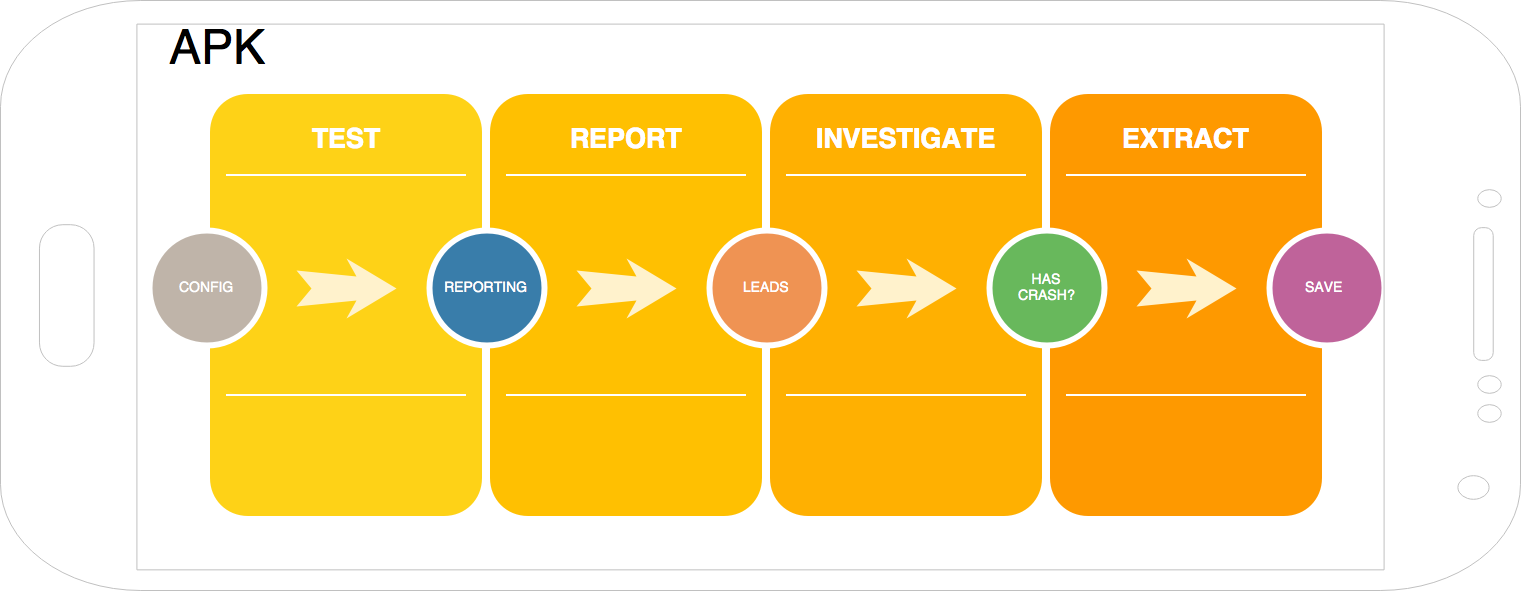
\includegraphics[width=\columnwidth]{imgs/apkprocess} 
%\caption{Four test steps performed by \toolname\ of an application}
%\label{fig: apkprocess}
%\end{figure}



\toolname\ can now repeat this entire process with the next application (\ie the next iteration in the loop inside the method \textit{testAllApp())}. This scenario is represented by the "yes" answer of the question \textit{"are there still apps in the dataset which have not been tested in this dataset cycle?"} in the figure \ref{fig: testingapproach}.
Once all the applications specified in the dataset have been tested exactly one time, \SessionLauncher\ can begin with the next iteration in its loop (listing ~\ref{lst:startsession}) and so start testing the whole dataset another time. 
This scenario, in turn, is described by the "no" answer of the question above. Indeed, the diagram \ref{fig: testingapproach} consequently starts the \textit{dataset cycle} again. 
This loop ends when the number of iterations reaches the one specified by the user. \\
In addition, during each test iteration and at the end of the whole testing session useful statistics are computed and written into external excel files, using the components \textsc{OnGoingCalculator} and \textsc{FinalCalculator}. They use the pure Java library \textit{Apache POI}, for reading and writing files in Microsoft Office formats \cite{apachepoi}. 




\section{Clustering}
\label{tool: clustering}
%-----Toool------
%Before the explanation of the Clustering process can start, a premise must be made. \GIO{What premise?} All the classes that will be discussed below, refer to the class diagram represented in the figure~\ref{clustering}. 


%TODO aggiungere construttore in crash log passandogli gli argomenti
First of all, \toolname\ individuates the directory in which all the previously generated crash logs have been stored. This directory is indicated again in the \Config.\\  
As shown in the listing~\ref{lst: extractor}, \toolname\ loops all the crashes contained inside it and for each of them it calls the method \textit{extractCrashLog()}, in the \Extractor\ component. 

\begin{lstlisting}[caption=\Extractor\ code snippet converting crash files into CrashLog objects,label={lst: extractor}]
/**
* @class: Main
*/
CrashLogExtractor extractor = new CrashLogExtractor();
final String CRASH_CONTAINER = ConfigurationManager.getCrashContainerDirectory();
File[] crash_container = new File(CRASH_CONTAINER).listFiles();
for (File crash : crash_container) {
	extractor.extractCrashLog(crash);
}
\end{lstlisting} 
The method \textit{extractCrashLog()} converts simple crash log files stored inside a folder into \Crash\ Java-objects. 
Indeed, for each crash log file found inside the directory, the constructor of the \Crash\ class get instantiated and so a new object of this type gets created. Each time the constructor of the \Crash\ class gets invoked, it automatically creates the structure of the \Crash-object analogously to the structure of the real crash log file. \\
For instance, the crash log described in the listing \ref{lst: ringdroid} is converted into a \Crash-object represented in the listing~\ref{lst: crashobject}.
It is printed out using the trivial Java method \textit{toString()}, which  per default gives a String representation of the object in question.  

\begin{lstlisting}[caption=\Crash-object,basicstyle=\fontsize{6}{8}\ttfamily, label={lst: crashobject}]
Crash {
	crash_path = /Users/Lucas/Desktop/UZH/BA/CrashLogCollector/crash_log_com.ringdroid.txt
	packageName = com.ringdroid
	Short = android.database.StaleDataException
	Long = android.database.StaleDataException: Attempted to access a cursor after it has been closed.
	first_java_trace_line = android.database.StaleDataException: Attempted to access a cursor after it has been closed.
	trigger_method = [android.database.BulkCursorToCursorAdaptor.getCount(BulkCursorToCursorAdaptor.java:70)]
	trigger_class = BulkCursorToCursorAdaptor
	log_lines = [// CRASH: com.ringdroid (pid 20442), // Short Msg: android.database.StaleDataException, ...]
}
\end{lstlisting}
%	all_stack_trace_methods = [BulkCursorToCursorAdaptor, CursorWrapper, MergeCursor,
	 						  %CursorAdapter, AdapterView, AbsListView, ViewGroup, Handler, Looper, ActivityThread, 
	 						  %Method, ZygoteInit]
%augmented_stack_traces = [android, database, stale, attempted, access, cursor, closed, bulk, adaptor, count, wrapper , merge, widget, adapter]  
From the listing above we can observe how the \Crash-object has assumed the same structure as the crash log file. Indeed, it analogously describes the \textit{package name} to which the crash belongs, the \textit{short} and the \textit{long} explanations about the exception, the \textit{trigger method}, etc.
In addition to them, the \Crash-object stores a list of Strings containing the log words, where each position of the array is occupied by a different line. 
%-----------LUCENE------------
\paragraph{Preprocessing.}
In according to the approach explained in the section \ref{approach:clustering}, the words of the crash reports must be preprocessed (\textit{tokenized}) in order to prepare them to be compared to each other. 
In this sense, the \Crash\ class statically invokes the method \textit{tokenizeLine()} in the \Lucene\ class for each line contained in the crash log. Listing~\ref{lst: tokenizeline} shows how it concretely works. 
\begin{lstlisting}[caption=Each line inside the crash report is tokenized using \Lucene,label={lst: tokenizeline}]
/**
* @class: CrashLog
*/
for (String line : this.logLines) {
	LuceneTokenizer.tokenizeLine(line);
}
\end{lstlisting} 
To provide a concrete example, the following line, extracted from the crash report in listing~\ref{lst: ringdroid} is passed as argument to the method \textit{tokenizeLine()}: \vspace{-0.8cm}
\begin{center}
\framebox[1\width]{{\fontsize{6.5}{6}{ \texttt{
//\hspace*{0.6cm}at android.database.BulkCursorToCursorAdaptor.throwIfCursorIsClosed(BulkCursorToCursorAdaptor.java:64)}
}}} \par
\end{center}
The following two boxes show the various tokenization steps that are performed by \toolname.
\begin{enumerate}
\item \textbf{Lucene StandardTokenizer}\\ \vspace{0.3em}
\framebox[1\width]{{\fontsize{6.5}{6}{ \texttt{at}
}}}
\framebox[1\width]{{\fontsize{6.5}{6}{ \texttt{android}
}}}
\framebox[1\width]{{\fontsize{6.5}{6}{ \texttt{database}
}}}
\framebox[1\width]{{\fontsize{6.5}{6}{ \texttt{BulkCursorToCursorAdaptor}
}}}
\framebox[1\width]{{\fontsize{6.5}{6}{ \texttt{throwIfCursorIsClosed}
}}}
\framebox[1\width]{{\fontsize{6.5}{6}{ \texttt{BulkCursorToCursorAdaptor}
}}}
\framebox[1\width]{{\fontsize{6.5}{6}{ \texttt{java}
}}}
\framebox[1\width]{{\fontsize{6.5}{6}{ \texttt{64}
}}}
\item \textbf{\toolname\ CamelCase Tokenizer} \\ \vspace{0.3em}
\framebox[1\width]{{\fontsize{6.5}{6}{ \texttt{at}
}}}
\framebox[1\width]{{\fontsize{6.5}{6}{ \texttt{android}
}}} 
\framebox[\width]{{\fontsize{6.5}{6}{ \texttt{database}
}}}
\framebox[\width]{{\fontsize{6.5}{6}{ \texttt{Bulk}
}}}
\framebox[\width]{{\fontsize{6.5}{6}{ \texttt{Cursor}
}}} 
\framebox[\width]{{\fontsize{6.5}{6}{ \texttt{To}
}}}
\framebox[\width]{{\fontsize{6.5}{6}{ \texttt{Cursor}
}}}
\framebox[\width]{{\fontsize{6.5}{6}{ \texttt{Adaptor}
}}} 
\framebox[\width]{{\fontsize{6.5}{6}{ \texttt{throw}
}}}
\framebox[\width]{{\fontsize{6.5}{6}{ \texttt{If}
}}}
\framebox[\width]{{\fontsize{6.5}{6}{ \texttt{Cursor}
}}} 
\framebox[\width]{{\fontsize{6.5}{6}{ \texttt{Is}
}}}
\framebox[\width]{{\fontsize{6.5}{6}{ \texttt{Closed}
}}}
\framebox[\width]{{\fontsize{6.5}{6}{ \texttt{Bulk}
}}} 
\framebox[\width]{{\fontsize{6.5}{6}{ \texttt{Cursor}
}}}
\framebox[\width]{{\fontsize{6.5}{6}{ \texttt{To}
}}} 
\framebox[\width]{{\fontsize{6.5}{6}{ \texttt{Cursor}
}}} 
\framebox[\width]{{\fontsize{6.5}{6}{ \texttt{Adaptor}
}}} 
\framebox[\width]{{\fontsize{6.5}{6}{ \texttt{java}
}}} 
\framebox[\width]{{\fontsize{6.5}{6}{ \texttt{64}
}}} 



\item \textbf{\toolname\ LowerCase Tokenizer} \\ \vspace{0.3em}
\framebox[1\width]{{\fontsize{6.5}{6}{ \texttt{at}
}}}
\framebox[1\width]{{\fontsize{6.5}{6}{ \texttt{android}
}}} 
\framebox[\width]{{\fontsize{6.5}{6}{ \texttt{database}
}}}
\framebox[\width]{{\fontsize{6.5}{6}{ \texttt{bulk}
}}}
\framebox[\width]{{\fontsize{6.5}{6}{ \texttt{cursor}
}}} 
\framebox[\width]{{\fontsize{6.5}{6}{ \texttt{to}
}}}
\framebox[\width]{{\fontsize{6.5}{6}{ \texttt{cursor}
}}}
\framebox[\width]{{\fontsize{6.5}{6}{ \texttt{adaptor}
}}} 
\framebox[\width]{{\fontsize{6.5}{6}{ \texttt{throw}
}}}
\framebox[\width]{{\fontsize{6.5}{6}{ \texttt{if}
}}}
\framebox[\width]{{\fontsize{6.5}{6}{ \texttt{cursor}
}}} 
\framebox[\width]{{\fontsize{6.5}{6}{ \texttt{is}
}}}
\framebox[\width]{{\fontsize{6.5}{6}{ \texttt{closed}
}}}
\framebox[\width]{{\fontsize{6.5}{6}{ \texttt{bulk}
}}} 
\framebox[\width]{{\fontsize{6.5}{6}{ \texttt{cursor}
}}}
\framebox[\width]{{\fontsize{6.5}{6}{ \texttt{to}
}}} 
\framebox[\width]{{\fontsize{6.5}{6}{ \texttt{cursor}
}}} 
\framebox[\width]{{\fontsize{6.5}{6}{ \texttt{adaptor}
}}} 
\framebox[\width]{{\fontsize{6.5}{6}{ \texttt{java}
}}} 
\framebox[\width]{{\fontsize{6.5}{6}{ \texttt{64}
}}} 
\end{enumerate}
As shown above, the crash log line gets firstly preprocessed using the \textit{StandardTokenizer} provided by \textbf{Lucene}.
Afterwards, \toolname\ for the reasons explained in the section \ref{approach:clustering} performs a further tokenization step, tokenizing the lines using an additional \textit{CamelCase tokenizer}. 
Finally, it uses a simply tokenizer to make the words lower case. 
This tokenization process is repeated for all lines of all crash reports stored in the directory. At the end of this process, each \Crash-object has its own set of preprocessed log lines (in the class diagram \ref{clustering}, represented by the list of Strings \textit{crashLogWords})

\paragraph{TF-IDF}
In order to follow the clustering approach described in the section \ref{approach:clustering}, \toolname\ creates for each crash log its correspondent vector space model. 
For this purpose, it makes use of the \textbf{Lucene} library again.
Indeed, the approach proposed by Lucene consists of (i) executing a indexation process with a set of Lucene documents, (ii) creating a term vector for each document (iii) computing for each term within the vector its tf-idf score. \\ 
The  diagram \ref{fig: indexingprocess} illustrates the main components of the Lucene indexation process.
\begin{figure}[tb]
\centering 
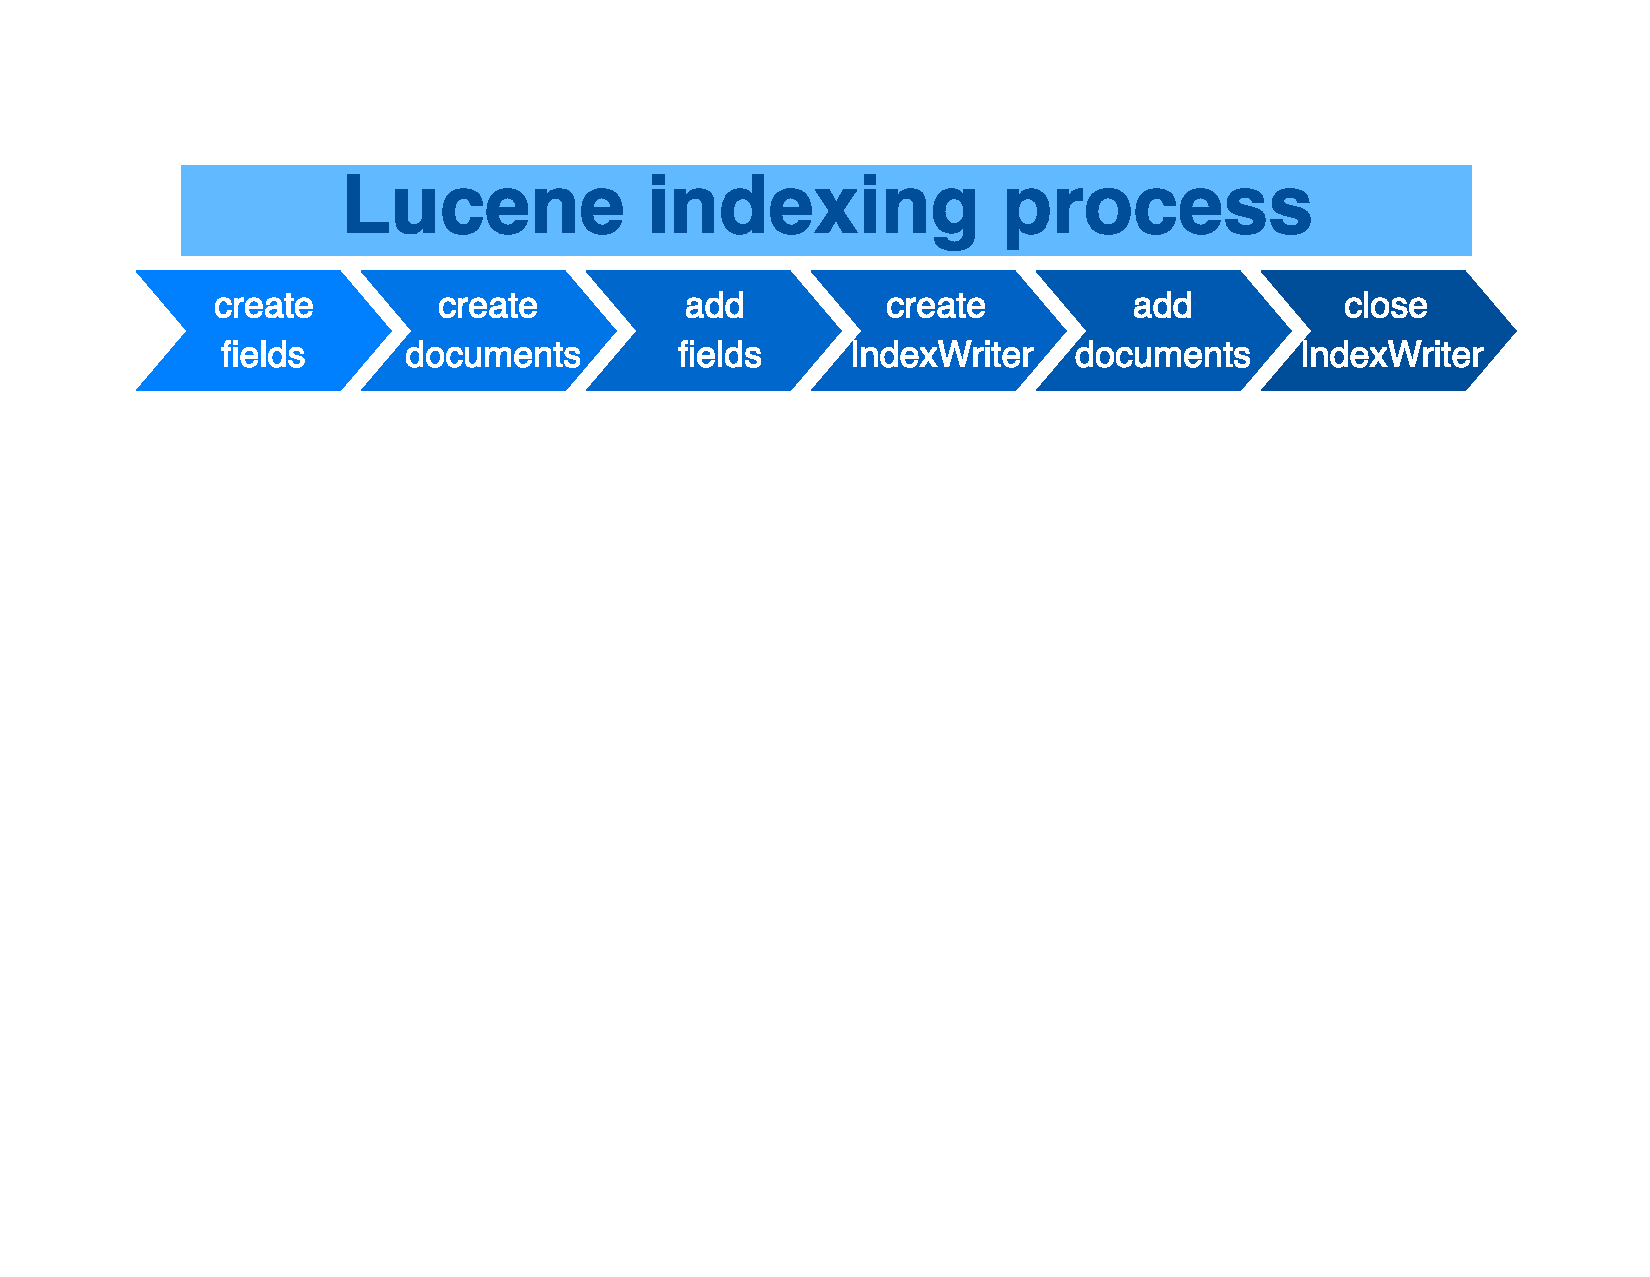
\includegraphics[width=\columnwidth]{diagrams/indexingProcess} 
\caption{Apache Lucene indexing process}
\label{fig: indexingprocess}
\end{figure}

\paragraph{Creating documents and adding fields.}
As a first step, \toolname\ generates a set of \textit{Lucene documents}. 
To do this, it goes through all previously created \Crash-objects and convert their preprocessed words into Lucene documents. Each document must contain its group of \textit{fields} in order to be indexed.
Therefore, when a new Lucene document is created, a set of fields must be set and enclosed inside it. 
A field can be viewed as a section of a document which can be optionally stored in the index \cite{lucenefield}. 
It has usually three components: \textit{name}, \textit{type} and \textit{content}. For each stored field, it is important to determine which type is best suited to the content that is going to be indexed. 
For instance, \toolname\ indexes documents which enclose \textit{text fields}, since they are already stored, tokenized and indexed \cite{lucenetextfield}. 
In order to be able to compute TF-IDF values for the indexed Lucene documents, \toolname\ must enable the property that they can have \textit{term vectors}, \ie they can store "a list of the document's terms and their number of occurrences in that document" \cite{lucenetermvector}. \\
The first steps of the Lucene indexing process can be summarized by the following code snippet, which is a simplified version of the \textit{createIndex()} method, illustrated in the diagram~\ref{clustering}.

\begin{lstlisting}[caption=\TFIDF\ describing the Lucene indexing process,label={lst: indexing}]
/**
* @class: TFIDFCalculator
*/
private void createIndex(List<CrashLog> crashLogs) throws IOException {
			// TODO: create IndexWriter
            for (CrashLog crash : crashLogs) {
                ArrayList<String> crash_log_words = crash.getSetOfWords();
                // type of field is set
                FieldType fieldType = new FieldType(TextField.TYPE_STORED); 
                // term vector is enabled
                fieldType.setStoreTermVectors(true); 
                // new document is created
                Document doc = new Document(); 
                for (String word : crash_log_words) {
                    // fields are added into the documents
                    doc.add(new Field(LConstants.FIELD_NAME, word, fieldType)); 
                }
                doc.add(new Field(LConstants.FIELD_ID, crash.getPath(), fieldType));
            }
\end{lstlisting} 
As shown in the listing above, \toolname\ goes through all the given crash logs and stores in a local list their preprocessed log words. 
Afterwards, the field type \textit{TextField} is selected (\textit{line 9}). 
In the next line, the above mentioned term vector property is enabled. 
Then, a new Lucene document is generated. 
At this point, \toolname\ goes through each preprocessed word and at each iteration adds the current word to a new field which has just been created (\textit{line 16}). 
The new field has a name, a content, \ie the word in question and a type, \ie the previously selected field type. 
Finally, the entire field is added to the document. 
At the end of the loop an additional field is added and used as ID for the document (in our case, the crash log path acts as unique attribute in the index). 

\paragraph{Creating IndexWriter and adding documents.}
In order to index Lucene documents, \toolname\ must generate an \textit{IndexWriter}. This because, this object acts as a core component for creating and updating indexes. 
First of all, \toolname\ creates an object of type \textit{IndexWriter}. However, the instantiating process of this class requires some supplementary configurations that must be passed to the constructor in order to create a new object of that type. 
These two information consist in (i) the directory where the index should point at and (ii) the Lucene \textit{Analyser} which is in charge of analysing the indexed documents. 
After the specification of these two information, a new object of type \textit{IndexWriter} can be created. 
Once created, all documents can be added to the index. At the end of the indexing process the writer must be closed.\\
The listing below complements the code snippet~\ref{lst: indexing} with the instantiation of the \textit{IndexWriter} class and consequentially with the addition of the documents to the index.  
\begin{lstlisting}[caption=\TFIDF\ describing the instantiation of an IndexWriter,label={lst: indexwriter}]
/**
* @class: TFIDFCalculator
*/
private void createIndex (List<CrashLog> crashLogs) throws IOException {
			// directory gets specified
		    FSDirectory dir = FSDirectory.open(new File("\Users\Lucas\Desktop\BA\Index").toPath());
		    // configuration is set
            IndexWriterConfig config = new IndexWriterConfig(new StandardAnalyzer());
            // IndexWriter gets instantiated 
            IndexWriter writer = new IndexWriter(dir, config);
	
            for (CrashLog crash : crashLogs) {
                ArrayList<String> crash_log_words = crash.getSetOfWords();
                FieldType fieldType = new FieldType(TextField.TYPE_STORED); 
                fieldType.setStoreTermVectors(true); 
                Document doc = new Document(); 
                for (String word : crash_log_words) {
                    doc.add(new Field(LConstants.FIELD_NAME, word, fieldType)); 
                }
                doc.add(new Field(LConstants.FIELD_ID, crash.getPath(), fieldType));
                // document are added to the index using an IndexWriter object
                writer.addDocument(doc);
   			}
                writer.close();
}
    
\end{lstlisting} 
As illustrated in the example above, the location where the index should point at can be inserted using the Lucene class \textit{FSDirectory} (\textit{line 6}). It is a base class for Directory implementations that store index files in the file system \cite{lucenefsdir}. 
Next line of code, the analyser which is used for analysing the Lucene documents is defined. 
This can made using the Lucene class \textit{IndexWriterConfig}, which holds all the configuration that is used to create an \textit{IndexWriter} (\textit{line 8}). \toolname\ defines again a \textit{StandardAnalyser}, the same used for preprocessing the crash logs.
Finally, a new \textit{IndexWriter} can be constructed per the previously configured settings. 
Once an \textit{IndexWriter} is created, all Lucene documents can be added to the index using a simple method called \textit{addDocument()}. At the end of the indexing process all preprocessed words contained inside the \Crash-objects have been converted into Lucene documents and have been indexed.


\paragraph{Computing TF-IDF scores.} 
At this point, the index has been created and each document has the possibility to store its vector of terms. 
Thus, TF-IDF values can now be computed for each word of each vector of each crash report. 
In this direction, \toolname\ invokes the \textit{computeScoreMap()} method in the \TFIDF\ class, which returns a hash map object. 
This hash map has as keys the unique locations of the crash logs, each one of them is associated with another hash map which contains the correspondent term vector.
Table~\ref{tbl: scoremap} shows the structure of the hash map, taking as a reference the crash log presented in the listing~\ref{lst: ringdroid}. 
\begin{table}[tb]
\centering
\caption{Structure of the hash map containing its term vector}
\label{tbl: scoremap}
\begin{tabular}{l|c|c|}
\hline
\multicolumn{1}{|c|}{{\color[HTML]{000000} \textit{\textbf{Crash log path (key)}}}}                                 & \multicolumn{2}{c|}{{\color[HTML]{000000} \textit{\textbf{HashMap (value)}}}} \\ \hline
\multicolumn{1}{|l|}{\textit{../Desktop/BA/CrashLogCollector/crash\_log1\_com.ringdroid.txt}} & {\textit{term (key)}}                   & { \textit{tfidf (value)}}                  \\ \hline
                                                                                                            & \hspace{0.7cm}exception\hspace{0.7cm}                             & \hspace{0.2cm}1.73\hspace{0.2cm}                                      \\ \cline{2-3} 
                                                                                                            & view                               & 5.12                                  \\ \cline{2-3} 
                                                                                                            & accessibility                         & 4.77                                  \\ \cline{2-3} 
                                                                                                            & crash                                 & 1.00                                  \\ \cline{2-3} 
                                                                                                            & scrollable                            & 1.92                                  \\ \cline{2-3} 
                                                                                                            & adapter                               & 2.44                                  \\ \cline{2-3} 
                                                                                                            & ringdroid                             & 1.00                                  \\ \cline{2-3} 
                                                                                                            & ...                             & ...                                  
\end{tabular}
\end{table}

As shown in the table~\ref{tbl: scoremap}, the terms which have the highest tf-idf relevance are \textit{accessibility} and \textit{view}. Indeed, they have a high term frequency in the currently scored crash log and a low document frequency in the entire collection. 
Terms such as \textit{crash} or \textit{ringdroid} have a low tf-idf weight. In fact, they are generic and irrelevant terms, since they don't give any useful information about the topic of the document. \\
%\toolname\ computes tf-idf scores for all vector terms of all crash logs. Once this processed is completed, the similarity between the set of crash logs stored inside the hash map can be computed.

\paragraph{Cosine similarity.} 
In order to state whether two crash logs refer to the same bug, \ie they can belong to the same group in the bucket, \toolname\ follows the approach described in the section \ref{approach:clustering}. 
Indeed, it computes a well-known similarity measure, \ie cosine similarity \cite{cosine} between different crash reports.
However, as a necessary preliminary step, the two vectors referring to the two different crash logs have first be \textit{normalized}. 
The \textit{normalization} process described in the approach (section \ref{approach:clustering}) is reported in the example shown in the table \ref{tbl: beforenormal} and \ref{tbl: afternormal}.
As illustrated, the vectors $A$ and $B$ after the normalization process have the same length and have been complemented with their missing words. 
\begin{table}[tb]
\centering
\caption{Vector terms $A$ and $B$ before normalization}
\label{tbl: beforenormal}
\begin{tabular}{ccllcc}
\cline{1-2} \cline{5-6}
\multicolumn{2}{|c|}{{\color[HTML]{000000} \textit{\textbf{Vector A}}}}     &  & \multicolumn{1}{l|}{} & \multicolumn{1}{c|}{{\color[HTML]{000000} \textit{\textbf{Vector B}}}} & \multicolumn{1}{c|}{}                \\ \cline{1-2} \cline{5-6} 
\multicolumn{1}{|c|}{\textbf{terms}} & \multicolumn{1}{c|}{\textbf{tf-idf}} &  & \multicolumn{1}{l|}{} & \multicolumn{1}{c|}{\textbf{terms}}                                    & \multicolumn{1}{c|}{\textbf{tf-idf}} \\ \cline{1-2} \cline{5-6} 
\multicolumn{1}{|c|}{handler}        & \multicolumn{1}{c|}{3.15}            &  & \multicolumn{1}{l|}{} & \multicolumn{1}{c|}{exception}                                         & \multicolumn{1}{c|}{1.73}            \\ \cline{1-2} \cline{5-6} 
\multicolumn{1}{|c|}{accessibility}  & \multicolumn{1}{c|}{1.7}             &  & \multicolumn{1}{l|}{} & \multicolumn{1}{c|}{handler}                                           & \multicolumn{1}{c|}{2.01}            \\ \cline{1-2} \cline{5-6} 
\multicolumn{1}{|c|}{crash}          & \multicolumn{1}{c|}{1.13}            &  & \multicolumn{1}{l|}{} & \multicolumn{1}{c|}{accessibility}                                     & \multicolumn{1}{c|}{4.77}            \\ \cline{1-2} \cline{5-6} 
\multicolumn{1}{|c|}{invoke}         & \multicolumn{1}{c|}{1.41}            &  & \multicolumn{1}{l|}{} & \multicolumn{1}{c|}{crash}                                             & \multicolumn{1}{c|}{1.00}            \\ \cline{1-2} \cline{5-6} 
\multicolumn{1}{|c|}{ringdroid}      & \multicolumn{1}{c|}{1.00}            &  & \multicolumn{1}{l|}{} & \multicolumn{1}{c|}{scrollable}                                        & \multicolumn{1}{c|}{1.92}            \\ \cline{1-2} \cline{5-6} 
                                     & \textbf{}                            &  & \multicolumn{1}{l|}{} & \multicolumn{1}{c|}{adapter}                                           & \multicolumn{1}{c|}{2.44}            \\ \cline{5-6} 
                                     &                                      &  & \multicolumn{1}{l|}{} & \multicolumn{1}{c|}{ringdroid}                                         & \multicolumn{1}{c|}{1.00}   \\ \cline{5-6} 
                                     &                                      &  &                       &                                                                        &                                     
\end{tabular}
\end{table}

\begin{table}[tb]
\centering
\caption{Normalized weighted vector terms $A$ and $B$}
\label{tbl: afternormal}
\begin{tabular}{|c|c|c|c|}
\hline
\multicolumn{2}{|c|}{{\color[HTML]{000000} \textit{\textbf{Vector A}}}} & \multicolumn{2}{c|}{{\color[HTML]{000000} \textit{\textbf{Vector B}}}} \\ \hline
\textbf{terms}                     & \textbf{tf-idf}                    & \textbf{terms}                    & \textbf{tf-idf}                    \\ \hline
\textbf{exception}                          & \textbf{0}                         & exception                         & 1.73                               \\ \hline
handler                            & 3.15                               & handler                           & 2.01                               \\ \hline
accessibility                      & 1.7                                & accessibility                     & 4.77                               \\ \hline
crash                              & 1.13                               & crash                             & 1.00                               \\ \hline
\textbf{scrollable}                         & \textbf{0}                         & scrollable                        & 1.92                               \\ \hline
\textbf{adapter}                            & \textbf{0}                         & adapter                           & 2.44                               \\ \hline
invoke                             & 1.41                               & \textbf{invoke}                            & \textbf{0}                         \\ \hline
ringdroid                          & 1.00                               & ringdroid                         & 1.00                               \\ \hline
\end{tabular}
\end{table}


\paragraph{Computing Cosine Similarity to create the bucket.}
Once the vector terms have been normalized, the cosine similarity among crash reports can be computed. In this direction, \toolname\ defines a threshold in the class \Oracle\,  which represents the tolerance for evaluating the similarity between two crash reports. Indeed, if the calculated cosine similarity among them is greater than the given limit, the two crash logs are considered to describe the same bug, \ie they will belong to the same bug group in the bucket. 

Concretely, \toolname\ invokes the method \textit{fillCrashLogBucket()}, which is in charge of comparing the crash logs, classifying them with the aim of filling the bucket. 
The bucket consists of a hash map, which has as keys a set of Strings which act as a labels for the entire bug group they represent. Each label, in turn, has its own list of \Crash-objects\, which have been considered by the \Oracle\ referring to the same bug.  \\
The bucketing process iterates all crash reports and it concretely works as follows: 
\begin{enumerate}
\item The method \textit{fillCrashLogBucket()} firstly extracts the first crash log in the list and insert it into the bucket, assigning to it the label of the first bug group. 
\item Starting from the second iteration, \toolname\ computes the cosine similarity between the current crash log and all crash logs which are placed at the first position in the list of the other bug groups. 
\item Whether all computed similarities are smaller than the threshold provided by the \Oracle\, means that there is no crash logs in the bucket already which can be considered the same as the current one. For this reason, \toolname\ creates a new bug group with a new label and insert into it the current crash log. \\
Otherwise, in the event that there is at least one computed similarity which is greater than the threshold, \toolname\ extracts the group inside the bucket which shows the highest similarity with the crash log and insert it into it.
In doing so, it gets added into the group which "resemble it more". 
\end{enumerate}
The \textit{BPMN}\footnote{Business Process Model and Notation} diagram \ref{bucketing} explains and summarizes the above mentioned bucketing process provided by \toolname. \\

\begin{figure}[tb]
\centering 
%	\vspace{-1.5mm} 
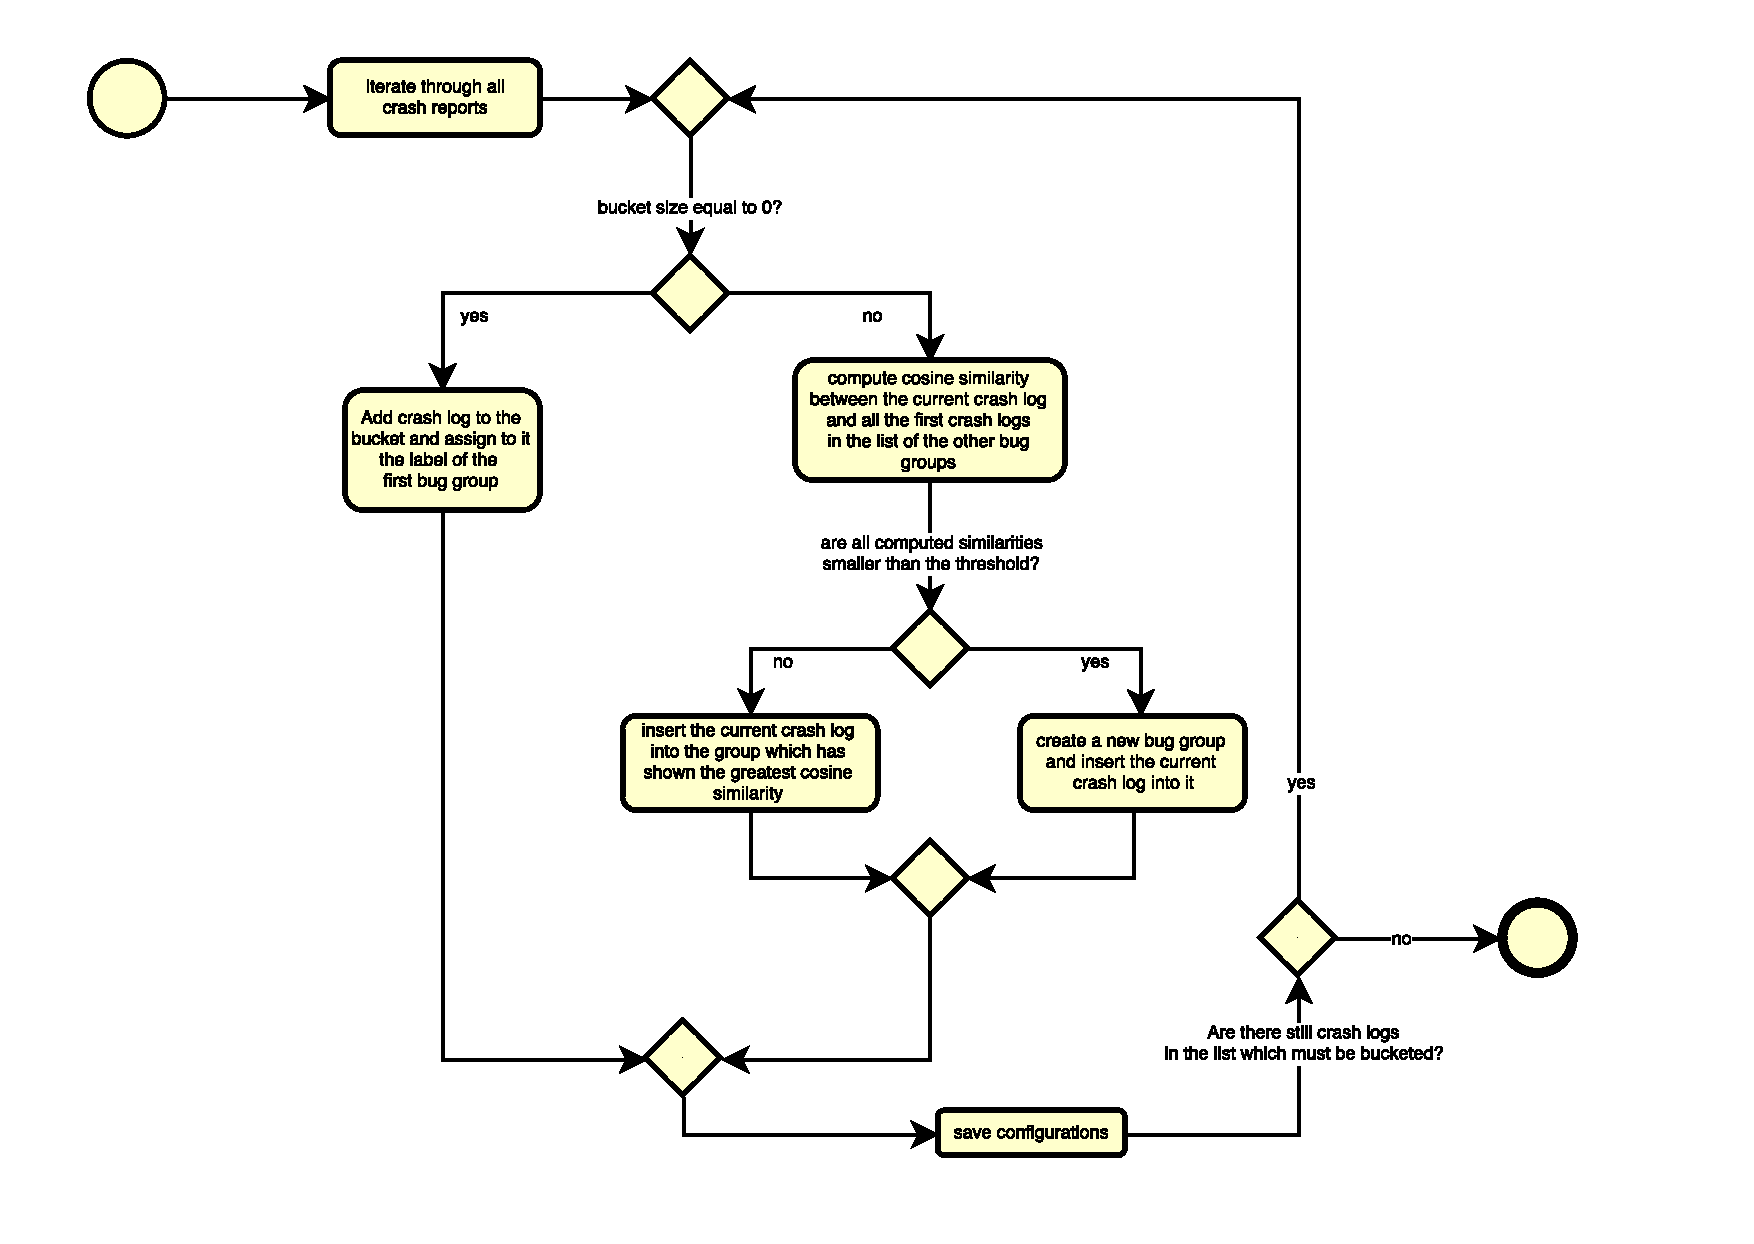
\includegraphics[width=\columnwidth]{diagrams/bucketingprocess.pdf} 
\caption{BPMN diagram describing the bucketing process}
\label{bucketing}
\end{figure}

At the end of the clustering phase, all crash logs collected in the testing phase have been systematically classified inside the bucket. 

%At the end of the bucketing process, \toolname\ saves the bucket and print it out. The clustering process is now completed. 
%conclusioni fare meglio


\section{Linking}
\label{tool: linking}
As mentioned in the introduction of the chapter \ref{chapter:approach}, the linking phase performed by \toolname\ is in charge of studying the complementarity between user feedback and the outcomes of automated testing tools, \ie the crash logs. 



\paragraph{Extracting user reviews.} 
The first step in the linking phase performed by \toolname\, is to read the dataset location, which contains the set of preprocessed and classified user reviews, specified in \Config.
Afterwards, \toolname\ uses the \ReviewC\ component illustrated in the diagram~\ref{linking}, in order to convert all user feedbacks located in the dataset to a set of Java-objects. 
To achieve this, each time \toolname\ finds a new review in the dataset, it instantiates the class \Review, creating a new object of that type. 
Afterwards, this object gets systematically inserted into a \textit{ReviewMap}, located in the \ReviewC\ class. 
This hash map has as keys a set of labels indicating the names of the packages for which the reviews have been submitted. Thus, each label is associated with its own list of \Review-objects. 
The table \ref{tbl: reviewmap} depicts a shortened version of the architecture of the \textit{ReviewMap}.
\begin{table}[tb]
\centering
\caption{Scheme of the Reviewmap}
\label{tbl: reviewmap}
\begin{tabular}{c|c|}
\hline
\multicolumn{1}{|c|}{\textit{\textbf{Package name (key)}}}    & \textit{\textbf{Review list (value)}} \\ \hline
\multicolumn{1}{|c|}{{\ul \textit{com.danvelazco.fbwrapper}}} & Review object 1                       \\ \hline
                                                              & Review object 2                       \\ \cline{2-2} 
                                                              & Review object 3                       \\ \cline{2-2} 
                                                              & ...                                   \\ \hline
\multicolumn{1}{|c|}{{\ul \textit{com.amaze.filemanager}}}    & Review object 1                       \\ \hline
                                                              & Review object 2                       \\ \cline{2-2} 
                                                              & ...                                   \\ \cline{2-2} 
\end{tabular}
\end{table}
At this point, \toolname\ has at disposal two different sources information, \ie the set of \textit{\Crash-objects }collected and classified inside the previously constructed bucket and a set of preprocessed and categorized \textit{user reviews}. \\
Before the beginning of the linking process, the set of preprocessed words belonging to each \Crash-object must be \textit{augmented} in according to the approach explained in the section \ref{approach:linking}. \\
In this direction, \toolname\ firstly extracts each \Crash-object from the bucket and then invokes for each of them the method 
\textit{augmentstackTrace()} in the \Crash\ class. 
Concretely, the augmenting process works as follows: 
\begin{enumerate}
\item As explained in the section \ref{approach:linking}, for each \Crash-object only the name and the cause of the raised exceptions are selected, \ie the String attribute \textit{firstJavaStackTraceLine}. Taking again as reference the crash log illustrated in the figure~\ref{lst: ringdroid}, the name and cause of the exception can be found at \textit{line 5}. 
After the preprocessing procedure has been completed, the line looks like the following: 
\begin{center}
\smallbreak
\emph{\small android, database, stale, attempted, access, cursor closed, bulk, adaptor, count }. 
\end{center} 
As you can see, the line has been already "stemmed and cleaned" using the method \textit{stemmAndCleanReports()} in the \textsc{Augmenter} class. 
This method preprocesses the reports expoiting the information retrivial techniques used by \textbf{INFUSA-TA}, explained at the beginning of the section \ref{approach:linking}.
Indeed, programming keywords such as "\textit{if}", "\textit{throw}" or "\textit{java}" and too short words such as "\textit{to}" or "\textit{at}" have been removed after the preprocessing procedure. 
\item After cleaning the reports, the remaining text is augmented with the source code methods included in the stack trace. In this direction, \toolname\ firstly extracts all methods present in the stack trace. To achieve this, it goes through all log lines in the method \textit{augmentStackTrace()} and for each line it compiles the regular expression positioned at \textit{line 7} in the listing \ref{lst: augmentstack}. 
\clearpage
\begin{lstlisting}[caption=Regular expression for extracting all methods from a stack trace,label={lst: augmentstack}]
/**
* @class: CrashLog
*/
public void augmentStackTrace()() {
        for (String line : this.logLines) {
            if (line.startsWith("// 	at") && line.contains(".java:")) {
            		String[] temp = line.split("\\(")[0].split("\\.");
            		String method = temp[temp.length-1];
            		this.stackTraceMethods.add(method);
            }
        }
        ...
}
\end{lstlisting}
The first if statement checks whether the current line belongs to the stack trace body, thus starting from the line number number 4 in the example~\ref{lst: ringdroid}. 
At \textit{line 7}, \toolname\ extracts only the method which is involved in the current line. 
For instance, the method which will be extracted from the following crash log line: 
\begin{center}
\smallbreak
\emph{\small android.database.BulkCursorToCursorAdaptor.throwIfCursorIsClosed\textbf{(}BulkCursorToCursorAdaptor.java:64\textbf{)}}
\end{center} 
will be
\begin{center}
\emph{throwIfCursorIsClosed}
\end{center} 
Indeed, the regular expression firstly splits the line by a \textit{round bracket} creating a local static array of Strings. Afterwards, it selects the first position in this array. So, it splits the just created array by a \textit{period}, forming a second array of Strings. 
This array is stored into the variable called \textit{temp} (\textit{line 7}).
Finally, it selects the last position of this latter. 
The figure below depicts the splitting process for the crash log line represented above: 
\begin{itemize}

\item \texttt{line.split({\color{blue}"\textbackslash\textbackslash("})} \\
\emph{android.database.BulkCursorToCursorAdaptor.throwIfCursorIsClose,\\ BulkCursorToCursorAdaptor.java:64)}


\item \texttt{line.split({\color{blue}"\textbackslash\textbackslash("})[0]} \\
\emph{android.database.BulkCursorToCursorAdaptor.throwIfCursorIsClose}

\item \texttt{String[] temp = line.split({\color{blue}"\textbackslash\textbackslash("})[0].split({\color{blue}"\textbackslash\textbackslash."})} 
{\color{brown}// {\small \texttt{length = 4} }}\\
\emph{android, \\database, \\BulkCursorToCursorAdaptor, \\throwIfCursorIsClose}

\item \texttt{String method = temp[temp.{\color{blue}length}-1]}
{\color{brown}// {\small \texttt{temp[3]} }}\\
\emph{throwIfCursorIsClose}

\end{itemize}
Once all methods present in the trace stack have been extracted, \toolname\ controls whether in the list of methods coming from the source code there are elements in common with those coming from the stack traces. 
In the event that there are, all additional words, \ie a list of keywords concerning that method in the source code, are added to the above illustrated \textit{firstJavaStackTraceLine}. 
Code snippet below summarizes the core of the \textit{augmenting} process: 
\begin{lstlisting}[caption=Augmenting a stack trace with methods coming from the source code,label={lst: sourcecode}]
/**
* @class: Augmenter
*/
public List<String> getAdditionalWordsFromSourceCode(){
		HashMap<String, String> methods = Augmenter.getMethodsFromCSV();
		List<String> augmentedStackTrace = convertToList(this.firstJavaStackTraceLine);
		methods.forEach((pMethod, additionalWords)-> {
			if (this.stackTraceMethods.contains(pMethod)) {
				augmentedStackTrace.add(additionalWords);
			}
		});
    return augmentedStackTrace;
}
\end{lstlisting}
First of all, the words coming from the source code are stored inside a local hash map called \textit{methods}.
This hash map has as keys a set of Strings, which represent the name of the methods found while parsing the source code. 
Their values consists of a set of Strings, each of them contains a list of additional words split by a white space.  
\textit{Line 7} goes through each key element in the hash map and whether \toolname\ notices that there is an element in common between the list of stack trace methods and those from the source code (\textit{line 8}), it adds the associated additional words to the variable \textit{augmentedStackTrace} (\textit{line 9}).
At the end of this process, the \textit{firstJavaStackTraceLine} has been converted into a variable called \textit{augmentedStackTrace} and possibly augmented with the set of additional words for those methods in common. This variable now looks like the following: 
\begin{center}
\smallbreak
\emph{\small android, database, stale, attempted, access, cursor closed, bulk, adaptor, count, \\{\color{red}sound, hear, context, supported, filename, rate, channels, launch, intent, title}, ... }
\end{center} 
\end{enumerate}
At this point, \toolname\ has at disposal a set of \textit{preprocessed} reviews and a set of \textit{augmented} stack traces. 
The final step provides the linking procedure using the \textit{asymmetric Dice} similarity coefficient described in the section \ref{approach:linking}. \\
First, \toolname\ reads the Dice threshold declared inside the \Linker\ class, which represents the minimal score the \textit{preprocessed reviews} and the \textit{augmented stack traces} must obtain in order to be considered as linked. 
In the approach described in section~\ref{approach:linking}, pairs of documents having a Dice score higher than \textbf{0.5} were considered as linked by the approach.
In order to compute that coefficient, \toolname\ passes as arguments in the constructor in the \Linker\ class the pairs of documents, both in the form of a list of Strings. 
Afterwards, \Linker\ invokes the method \textit{evaluateLinking()}, which refers to the \textit{Façade pattern}. 
Indeed, the \Facade\ component reproduces the design pattern \textit{Facade}, 
which provides a simplified interface for evaluating the asymmetric Dice. 
Figure \ref{lst: facade} shows how it concretely works. 
\clearpage



\begin{lstlisting}[caption=\Facade implementing the design pattern \textit{Facade},label={lst: facade}]
/**
* @class: SimilarityMetricsFacade
* @return a double value representing the similarity between the given texts
*/
public static double evaluateAsimmetricDiceIndex(List<String> pReview, List<String> augmentedLog) {
        return AsimmetricDiceIndex.computeAsimmetricDiceIndex(pReview, augmentedLog);
}
\end{lstlisting}
After defining how the Dice coefficient is computed, \toolname\ must just go through all \Crash-objects, extracts for each of them its \textit{augmentedStackTrace} variable mentioned above. Then, iterates the whole set of \textit{preprocessed reviews} stored in the \textit{ReviewMap} illustrated in the table \ref{tbl: reviewmap}, and computes for each review the Dice coefficient among it and the \textit{augmentedStackTrace} variable. 
Finally, if the Dice score results greater than the threshold (in our case, 0.5), \toolname\ writes the correspondent \textit{review ID} with its set of preprocessed words and the set of words representing the augmented stack trace of the current crash log into an external \textit{csv}-File. To achieve this, it uses the component \Writer\, located in the package \textit{Utilities}. 
At the end of the entire linking process, \toolname\ writes some metadata into the \textit{csv}-File such as the date, the number of linked reviews, etc. 
The figure~\ref{lst: linkingprocess} shows a simplified code snippet representing the linking procedure described above. 
\begin{lstlisting}[caption=Linking process,label={lst: linkingprocess}]
/**
* @class: Main
*/
public void performLinking() {
	crashLogBucket.forEach((crash_log_location, crashlogs) -> {
		for (CrashLog crashLog : crashlogs) {
			 List<Review> reviewList = reviewMap.get(crashLog.getPackageName());
			 for (Review review: reviewList) {
			 	 List<String> preprocessedReview = review.getPreProcessedReview();	
			 	 List<String> augmentedStackTrace = crashLog.getAugmentedStackTraces();
			 	 double diceIndex = SimilarityMetricsFacade.evaluateAsimmetricDiceIndex(preProcessedReview, augmentedStackTrace);
			 	 if (diceIndex >= DICE_THRESHOLD) {	 
			 	 String content +=	"review_id:   " + review.getId() + ", "
	                                  + "\n preprocessed_review:   " + preProcessedReview.toString() + ", "
	                                  + "\n augmented_stack_trace:  " + augmentedStackTrace.toString() + ", "
	                                  + "\n dice score:    " + diceIndex + "\n\n";                     
			 	}
			}
		}
	}
	Writer.writeOnFile(content, Paths.get("linking_results.csv");
}
\end{lstlisting}
First, the list of crash logs stored for each bug group in the bucket gets iterated (\textit{line 5-6}). 
Afterwards, the correct list of review is individuated by specifying the package name of the crash log (\textit{line 7}). This is possible because the \textit{reviewMap} has a set of keys the name of packages for which the reviews have been submitted. 
Then, each \textit{Review} in the just created \textit{reviewList} gets iterated in the \textit{line 8}.
At this point, two list of Strings store the preprocessed words of the current review as well the augmented stack trace of the current crash log (\textit{line 9-10}.
Later, using the \Facade\ component the Dice score among the pairs of documents is computed (\textit{line 11}). 
\textit{Line 12} checks whether the calculated coefficient is greater thatn the threshold. 
If this is the case, the \textit{content} String (\textit{line 13}) is updated with 
the \textit{review id}, the set of words indicating the preprocessed review and finally the augmented stack trace. 
At the end of the entire linking procedure (\textit{line 21}), the \textit{content} String is written into an external file located at the specified \textit{path}.

\begin{figure}[tb]
\centering 
%	\vspace{-1.5mm} 
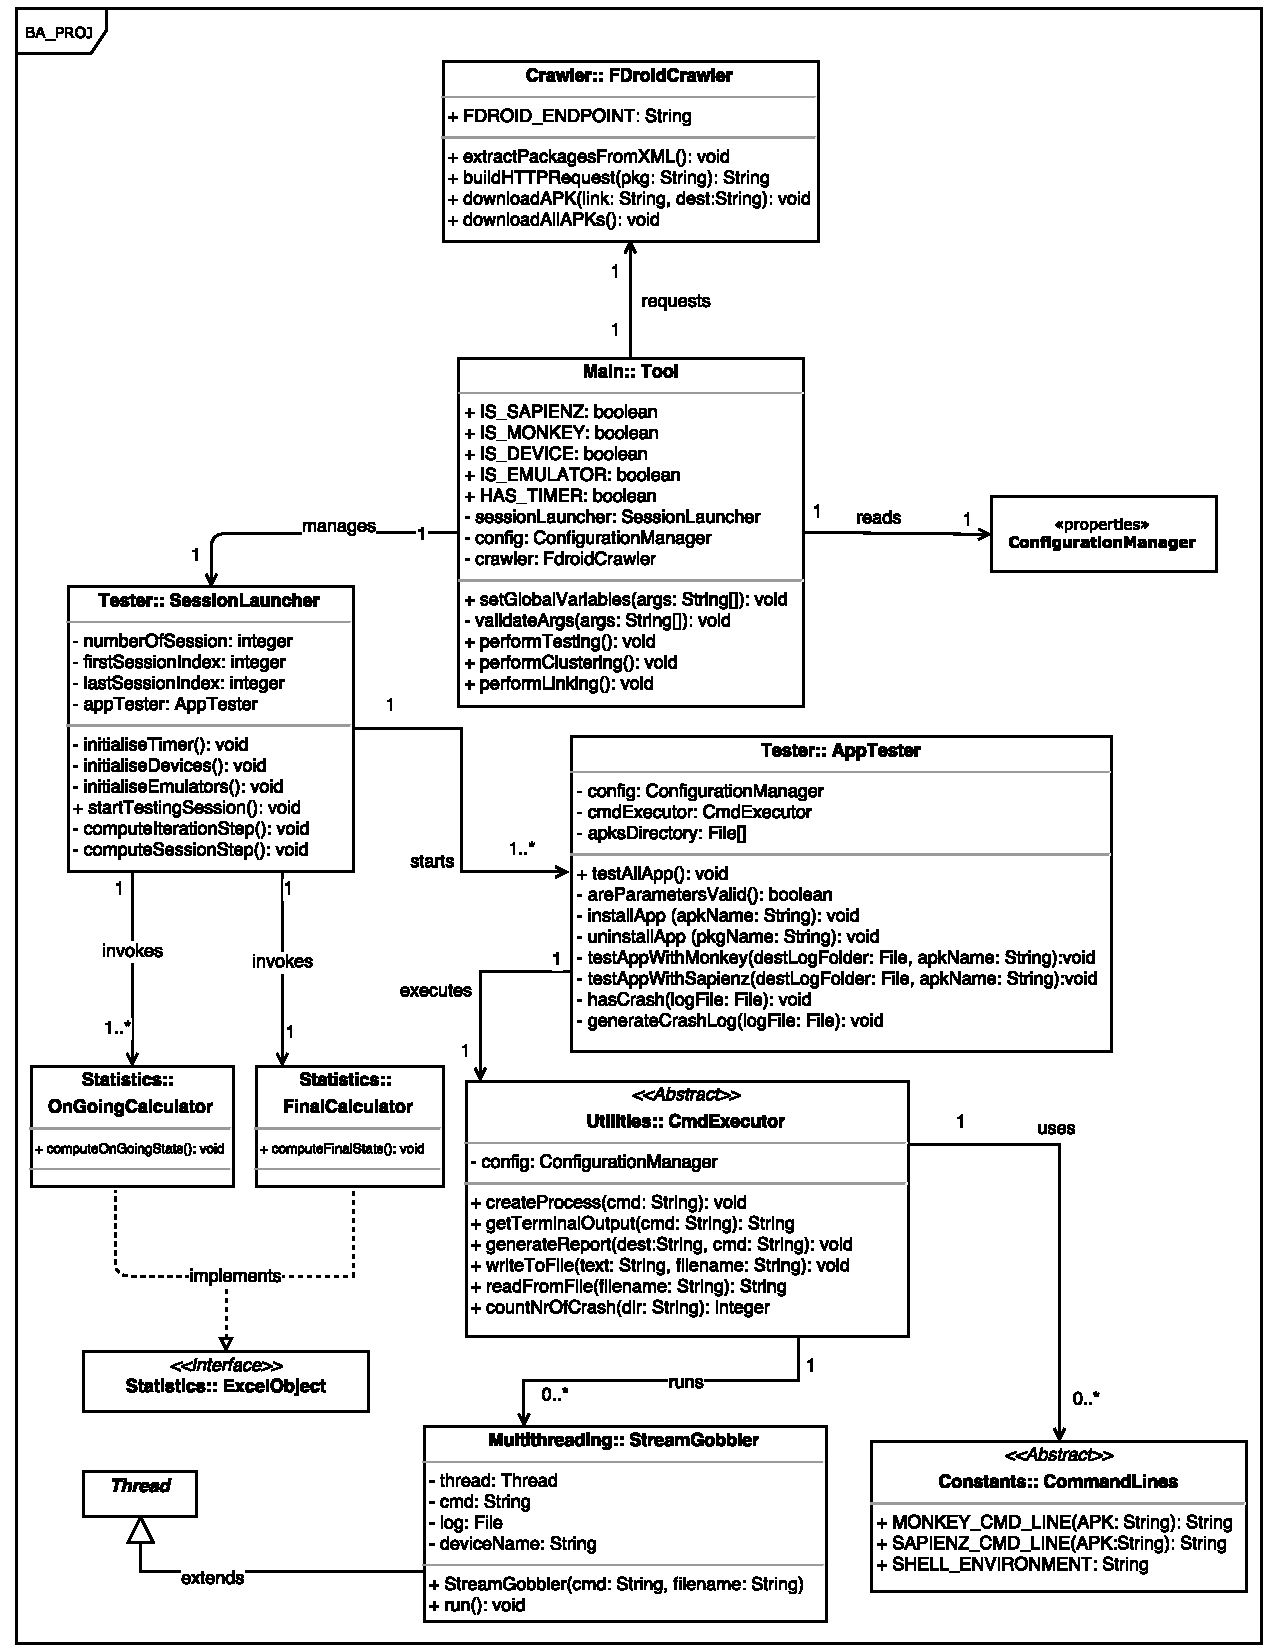
\includegraphics[width=\columnwidth]{diagrams/testing.pdf} 
\caption{Class Diagram of the testing part of the tool }
\label{testing}
\vspace{-3mm} 
\end{figure}


\begin{figure}[t]
\centering 
%	\vspace{-1.5mm} 
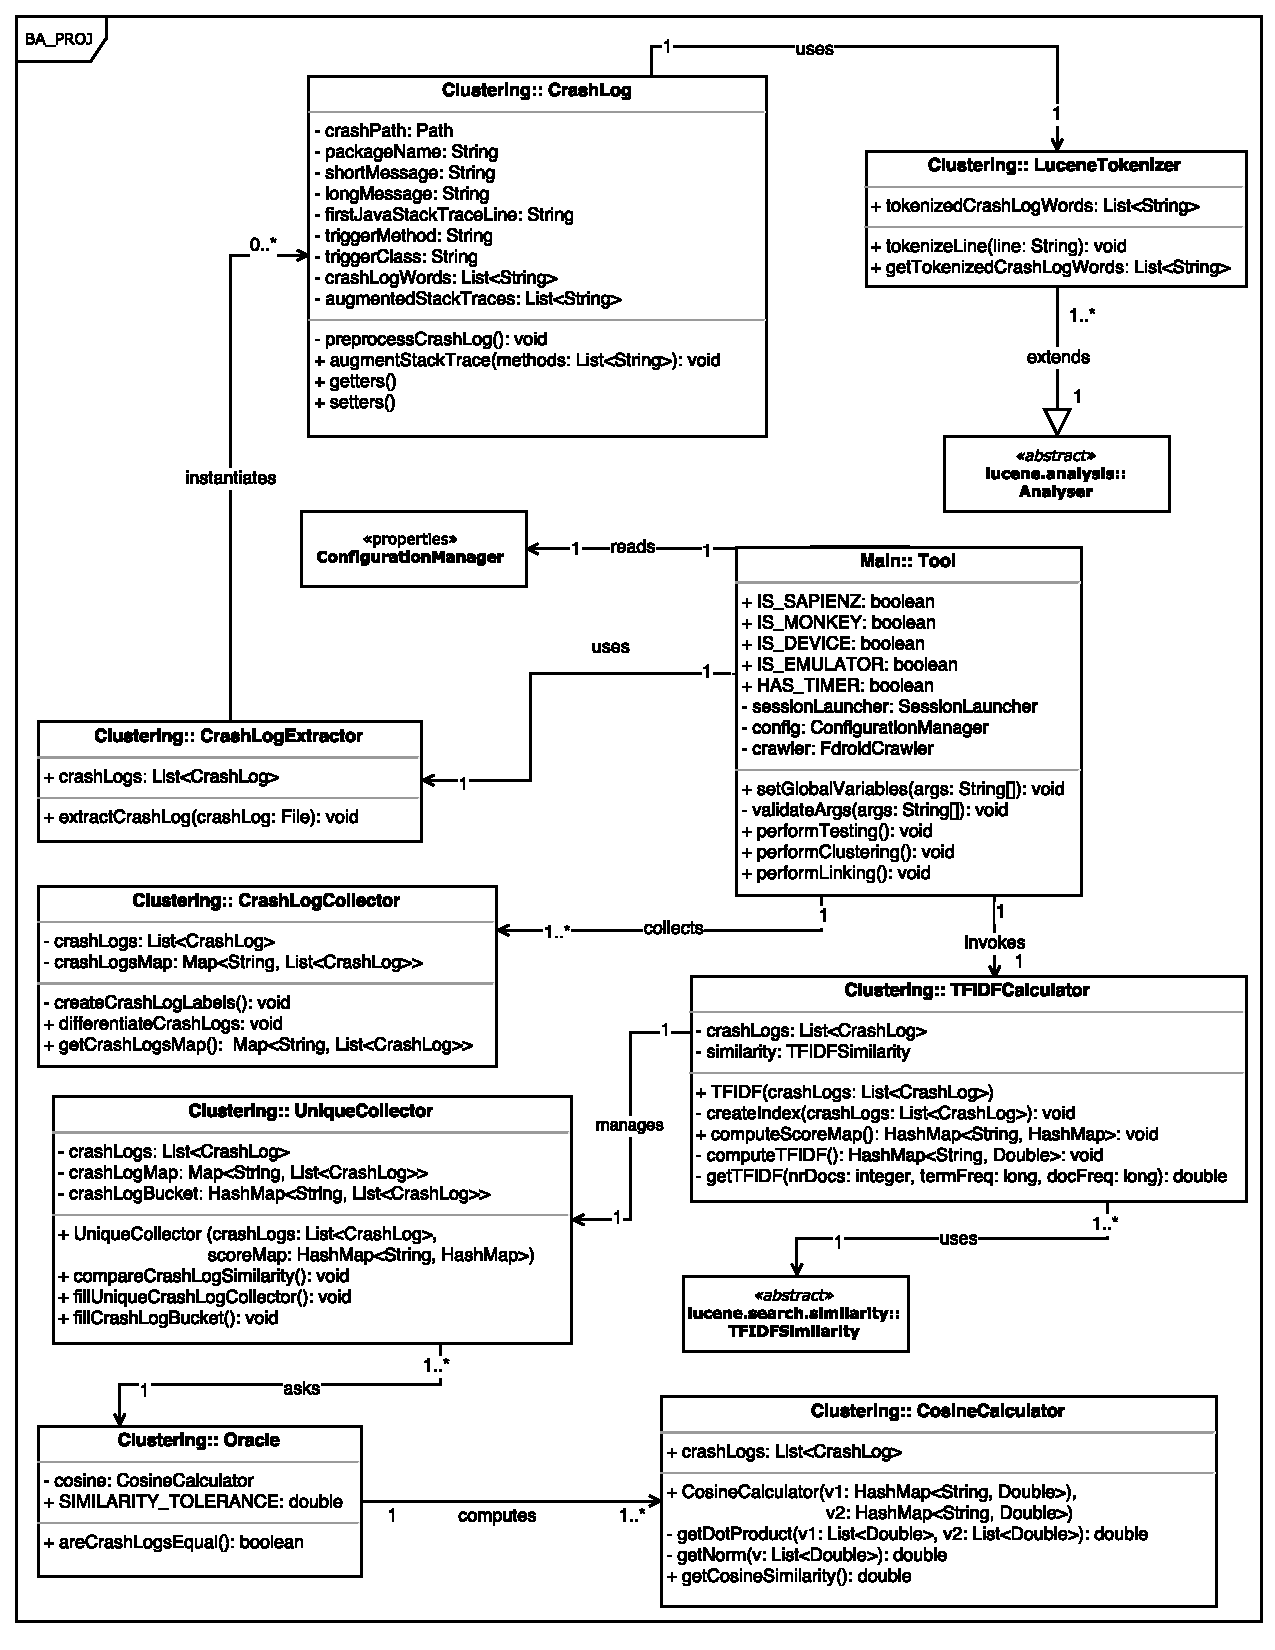
\includegraphics[width=\columnwidth]{diagrams/clustering.pdf} 
\caption{Class Diagram of the clustering part of the tool }
\label{clustering}
\vspace{-3mm} 
\end{figure}


\begin{figure}[t]
\centering 
%	\vspace{-1.5mm} 
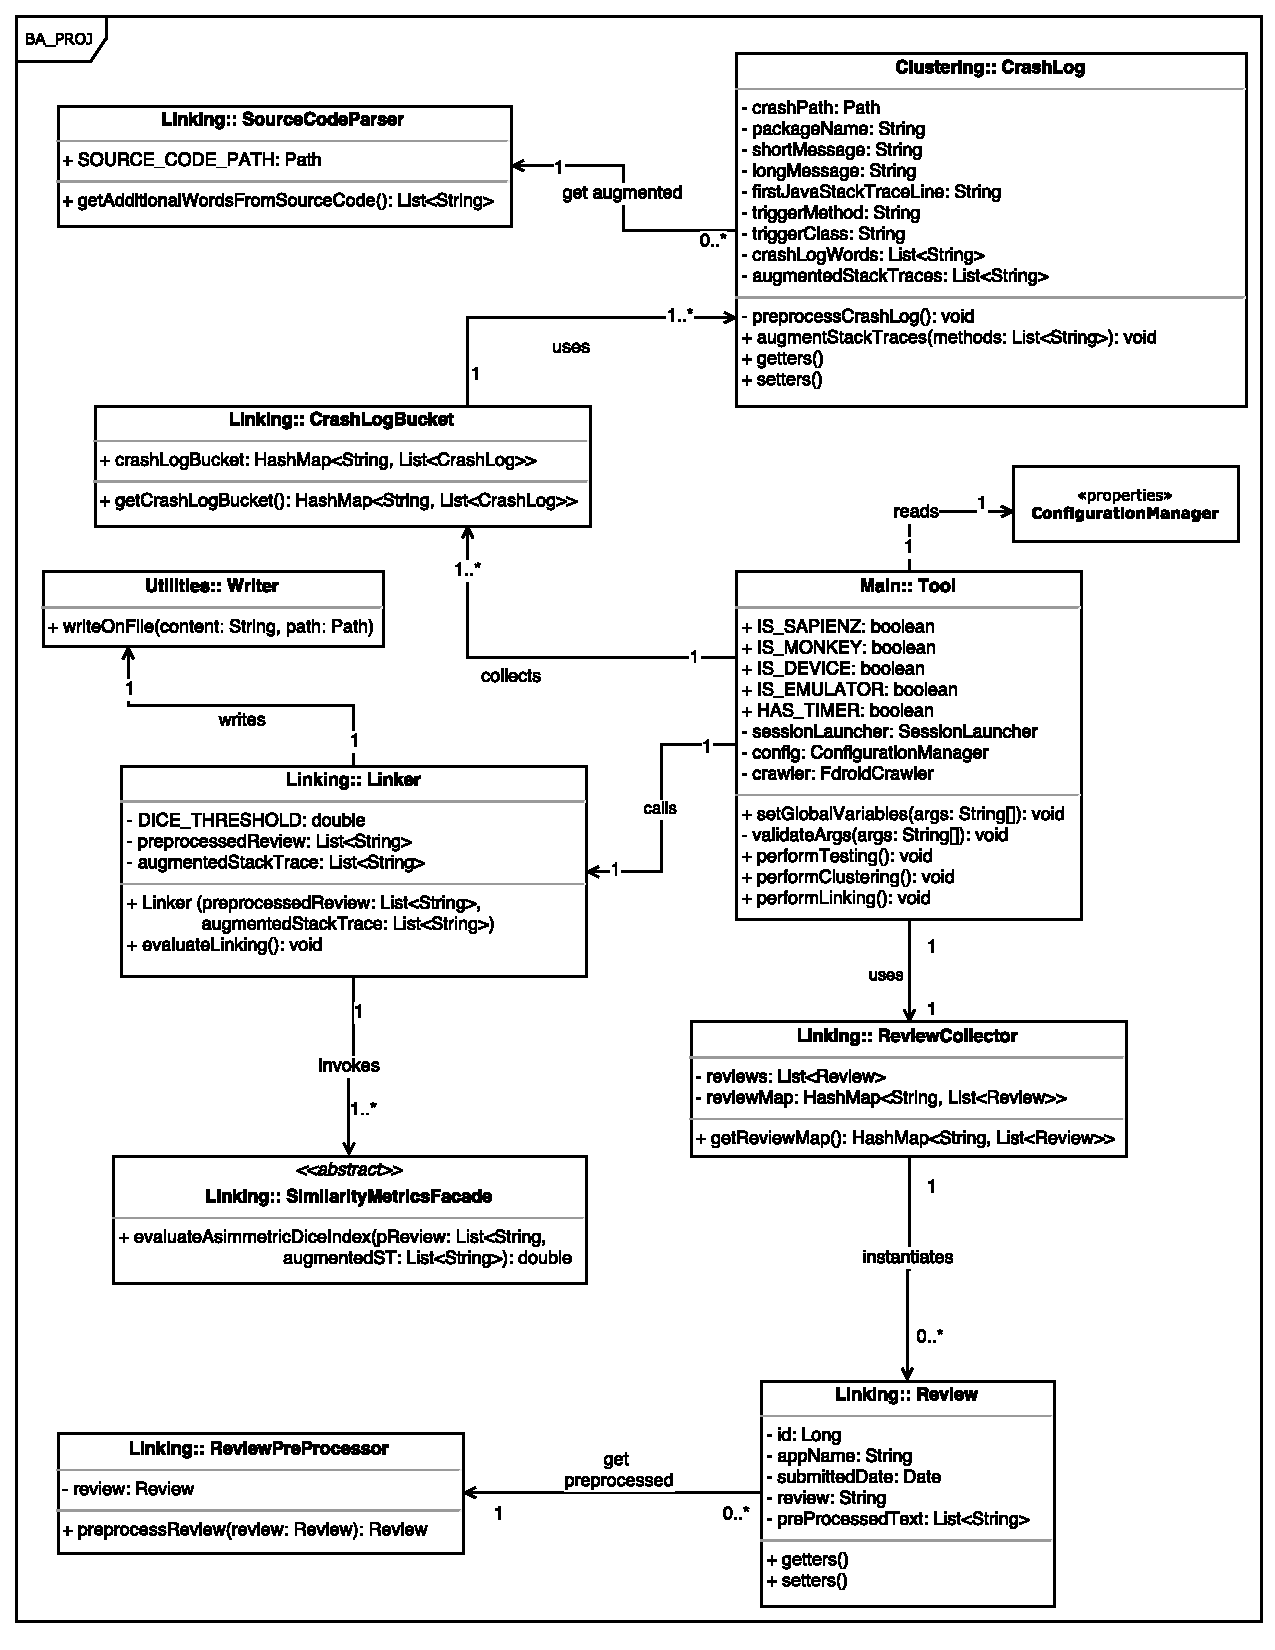
\includegraphics[width=\columnwidth]{diagrams/linking.pdf} 
\caption{Class Diagram of the linking part of the tool }
\label{linking}
\vspace{-3mm} 
\end{figure}


\section{Installation and usage of \toolname}
\toolname\footnote{the source code of \toolname\ is available at \toolurl } is still in a experimental stage. It has been fully tested uniquely with \textit{Android 4.4} and \textit{Mac OS 10.11}. 
Augmenting the compatibility of it with multiple operating systems is plan of my future agenda. 

\subsection{General Configuration}
First of all, in order to be able to use \toolname\ some external components must be installed and configured. 
The following shows the environment configurations that must be applied (they must be sequentially installed).
\begin{itemize}
\item \textbf{Brew} \\
Brew \cite{brew} is a manager for installing the missing packages for Mac OS. 
It can be installed running the following command line on a Mac OS: 
{\scriptsize
\begin{center}
\fbox{
\texttt{\$ /usr/bin/ruby -e "\$(curl -fsSL https://raw.githubusercontent.com/Homebrew/install/master/install)"
}
}
\end{center}
}%
\item \textbf{Android SDK Platform-Tool}\\
In order to easily install the Android SDK Platform-Tools component, which is required for launching \sapienz and \monkey just download and install \textit{Android Studio}, the official IDE for Android \cite{androidstudio}. 
The download link can be found at:  
\begin{center}
\url{https://developer.android.com/studio/index.html}
\end{center}
\item \textbf{pip} \\
Pip is a manager for installing python packages on a Mac OS. It is needed for installing some python dependencies used by \textsc{Sapienz}.  
It can be easily installed running the following command line: 	
\begin{center}
\fbox{
\texttt{\$brew install pip}
}
\end{center}
\begin{center}
or if it fails
\end{center}
\begin{center}
\fbox{
\texttt{\$ sudo easy\_install pip}
}
\end{center}

\end{itemize}

\subsection{Sapienz Environment Configuration}
In order to be able to perform a testing session using \sapienz, the \textit{emulators} respectively the attached \textit{devices} must have installed the \textbf{API 19} level (version code \textit{KitKat}) \cite{api19}. 
The following describes the configurations steps which have to be performed for using \textsc{Sapienz}. 
\begin{itemize}
\item\textbf{Environment variables} \\ 
Include the following $aapt$ path as environment variable in the bash profile:
\begin{center}
\fbox{
\texttt{/Users/<user\_name>/Library/Android/sdk/build-tools/19.x.x}
}
\end{center}

\item \textbf{Python dependencies} \\
Install some required python \textit{dependencies} using the \textit{requirements.txt} file located in the \sapienz\ directory: 
\begin{center}
\fbox{
\texttt{\$ sudo pip install -r requirements.txt}
}
\end{center}

\item\textbf{Python version} \\
The adequate python \textit{version}(\textit{2.7}) must be installed. 
Despite the correct version is installed, there may be a problem with the installation of the python dependencies. 
If that were the case, the following command line must be executed:  
\begin{center}
\fbox{
\texttt{\$ brew install python}
}
\end{center}
\end{itemize}
\subsection{Monkey Environment Configuration}
The only requirement to use monkey is that the package of \textit{Android SDK Platform-Tool} has been successfully installed.

\subsection{Settings}
%TODO far riferimento dove è presentato il config file a questa sezione per la descrizione dei testing parameters 
\label{usage: settings}
In order to start a testing session a set of specifications must be declared in the \Config\ file. 
This file configures the initial settings and the set of all parameters that will be processed by \toolname\ during the testing process. 
It is located in the \toolname\ source code and is renamed as \textit{config.properties}.
The most important properties have been already presented in the figure \ref{lst: config}.
In this sense, the following provides a detailed description about the testing parameters presented in the figure \ref{lst: config} \cite{monkey, sapienz}: 
\begin{itemize}
\item \textsc{Monkey}
\begin{itemize}
\item VERBOSITY ([\textit{-v, -v-v-v}]) \\
It defines the verbosity of the log. Each additional \textit{-v} increases the verbosity level. 
\item RANDOM\_EVENTS (\textit{int})\\
Number of random events that will be generated by \monkey\ in the testing cycle of a single \textit{APK}.
\item DELAY\_BETWEEN\_EVENTS (\textit{millisec})\\
It inserts a delay between the above specified number of random events. 
\item PERCENTAGE\_TOUCH\_EVENTS (\textit{int}, [0,100])\\
It adjusts the percentage of \textit{touch} events of the total number of events (\eg down-up events in the screen) 
\item PERCENTAGE\_SYSTEM\_EVENTS (\textit{int}, [0,100])\\
It adjusts the percentage of \textit{system} events of the total number of events (\eg volume controls) 
\item PERCENTAGE\_MOTION\_EVENTS (\textit{int}, [0,100])\\
It adjusts the percentage of \textit{motion} events of the total number of events (\eg random movements) 
\item IGNORE\_CRASHES (\textit{boolean}, [true,false])\\
It defines whether \monkey stops when a crash or an unhandled exception occurs. 
\end{itemize}
\item \textsc{Sapienz}
\begin{itemize}
\item SEQUENCE\_LENGTH\_MIN (\textit{int})\\
Minimum number of events that will be generated for each \sapienz cycle. 
\item SEQUENCE\_LENGTH\_MAX (\textit{int})\\
Maximum number of events that will be generated for each \sapienz cycle. 
\item SUITE\_SIZE (\textit{int})\\
The number of chromosomes (\ie test cases) that an individual (\ie test suite) owns. 
\item POPULATION\_SIZE (\textit{int})\\
Numbers of individuals in the population in the genetic algorithm. 
\item OFFSPRING\_SIZE (\textit{int})\\
The numbers of elements the offspring has in the whole test suite variation operator. 
\item GENERATION (\textit{int})\\
It sets the maximum generation number. 
\item CXPB (\textit{double}, [0,1])\\
It defines the crossover probability used by the genetic algorithm. 
\item MUTPB (\textit{double}, [0,1])\\
It defines the mutation probability used by the genetic algorithm. 
\end{itemize}
\end{itemize}

In addition to them, the following specifications must be inserted: 
\begin{itemize}
\item \textsc{EMULATOR\_NAME} \\
The name of the emulator on which the tests will be performed;
\item \textsc{AVD\_BOOT\_DELAY} (\textit{sec})\\
This time indicates how many seconds \toolname\ has to \textit{wait}, when the attached devices or the emulators get rebooted;
\item \textsc{TIME\_UNIT} (\textit{sec, min, hours})\\
It specifies the time unit recognized by the following \textit{timeouts}; 
\item \textsc{MONKEY\_TIMEOUT} \\
It indicates after how long the testing cycle of a single \textit{APK} tested with \monkey\ gets automatically interrupted so that the testing of the next app can start. These time frames can be very useful since there may happen that some devices, after generating a very large number of \textit{UI events} are not longer able to process new incoming events, freezing the entire Android system. 
\item \textsc{SAPIENZ\_TIMEOUT} \\
Same as above, only for \textsc{Sapienz}.
\item \textsc{ADB\_EXEC\_DIR}\\
It indicates the location of the executable file \textit{abd} (Android Debug Bridge), a command-line tool which facilitates the communication between the user and the Android OS. 
\end{itemize}

\subsection{\toolname\ usage}
After specifying settings and parameters in the \Config\ file, \toolname\ is ready to be started. 
The line below shows the usage of the \toolname\ command-line: 
\begin{center}
\fbox{
\small{
\texttt{\$ java -jar BECLOMA.jar [{\color{blue}-emulator} | {\color{blue}-device}] 
[{\color{blue}-monkey} | {\color{blue}-sapienz}] [timer]
}
}
}
\end{center}
The table \ref{tbl: toolarguments} lists all of the supported \toolname\ arguments and explains their meaning. 
\begin{table}[tb]
\centering
\caption{Command-line arguments supported by \toolname}
\label{tbl: toolarguments}
\begin{tabular}{|l|l|}
\hline
\rowcolor[HTML]{EFEFEF} 
\multicolumn{1}{|c|}{\cellcolor[HTML]{EFEFEF}\textbf{Supported arguments}} & \multicolumn{1}{c|}{\cellcolor[HTML]{EFEFEF}\textbf{Description}}        \\ \hline
\textit{-device}                                                           & Performs the testing on a physical attached android device               \\ \hline
\textit{-emulator}                                                         & Performs the testing on a virtual specified android emulator             \\ \hline
\textit{-monkey}                                                           & The dataset will be tested using monkey                                  \\ \hline
\textit{-sapienz}                                                          & The dataset will be tested using sapient                                 \\ \hline
\textit{-timer}                                                            & Optional.  Starts a timer for a better overview during a testing session \\ \hline
\end{tabular}
\end{table}
  









































